\let\negmedspace\undefined
\let\negthickspace\undefined
\documentclass[journal]{IEEEtran}
\usepackage[a5paper, margin=10mm, onecolumn]{geometry}
%\usepackage{lmodern} % Ensure lmodern is loaded for pdflatex
\usepackage{tfrupee} % Include tfrupee package

\setlength{\headheight}{1cm} % Set the height of the header box
\setlength{\headsep}{0mm}     % Set the distance between the header box and the top of the text

\usepackage{gvv-book}
%\usepackage{gvv}
\usepackage{cite}
\usepackage{amsmath,amssymb,amsfonts,amsthm}
\usepackage{algorithmic}
\usepackage{graphicx}
\usepackage{textcomp}
\usepackage{xcolor}
\usepackage{txfonts}
\usepackage{listings}
\usepackage{enumitem}
\usepackage{mathtools}
\usepackage{gensymb}
\usepackage{comment}
\usepackage[breaklinks=true]{hyperref}
\usepackage{tkz-euclide} 
\usepackage{listings}
\usepackage{gvv}                                        
\def\inputGnumericTable{}                                 
\usepackage[latin1]{inputenc}                                
\usepackage{color}                                            
\usepackage{array}                                            
\usepackage{longtable}                                       
\usepackage{calc}                                             
\usepackage{multirow}                                         
\usepackage{hhline}                                           
\usepackage{ifthen}                                           
\usepackage{lscape}
\begin{document}

\bibliographystyle{IEEEtran}

\title{5.2.22}
\author{EE25BTECH11019 - Darji Vivek M.}
{\let\newpage\relax\maketitle}

\renewcommand{\thefigure}{\theenumi}
\renewcommand{\thetable}{\theenumi}
\setlength{\intextsep}{10pt}
\numberwithin{figure}{enumi}
\renewcommand{\thetable}{\theenumi}

\textbf{Question}:\\
Solve for the system of linear equations:
\begin{align*}
    \sqrt{2}x+\sqrt{3}y=0\\
    \sqrt{3}x-\sqrt{8}y=0
\end{align*}

\solution \\
Let us solve the given question theoretically and then verify the solution computationally.\\
\\
The equation of lines given,
\begin{align}
    \myvec{\sqrt{2}&&\sqrt{3}}\vec{x}=0 \quad \myvec{\sqrt{3}&&-\sqrt{8}}\vec{x}=0
\end{align}
\begin{align}
    \therefore \myvec{\sqrt{2}&&\sqrt{3}\\\sqrt{3}&&-\sqrt{8}}\vec{x}=\myvec{0\\0}
\end{align}
Forming an augmented matrix,
\begin{align}
    \augvec{2}{1}{\sqrt{2}&\sqrt{3}&0\\\sqrt{3}&-\sqrt{8}&0}
\end{align}
Upon doing row reduction,
\begin{align}
\begin{aligned}
     \augvec{2}{1}{\sqrt{2}&\sqrt{3}&0\\\sqrt{3}&-\sqrt{8}&0}
     \xleftrightarrow{\,R_2 \gets R_2- \frac{\sqrt{3}}{\sqrt{2}} \times R_1}
     \augvec{2}{1}{\sqrt{2}&\sqrt{3}&0\\0&\left(-\sqrt{8}-\frac{3}{\sqrt{2}}\right)&0}  
     \xleftrightarrow{\,R_1 \gets R_1+ 0 \times R_2}
     \augvec{2}{1}{\sqrt{2}&\sqrt{3}&0\\0&\left(-\sqrt{8}-\frac{3}{\sqrt{2}}\right)&0}
\end{aligned}
\end{align}
\begin{align}
    \implies \vec{x}=\myvec{0\\0}
\end{align}

 \begin{figure}[H]
     \centering
     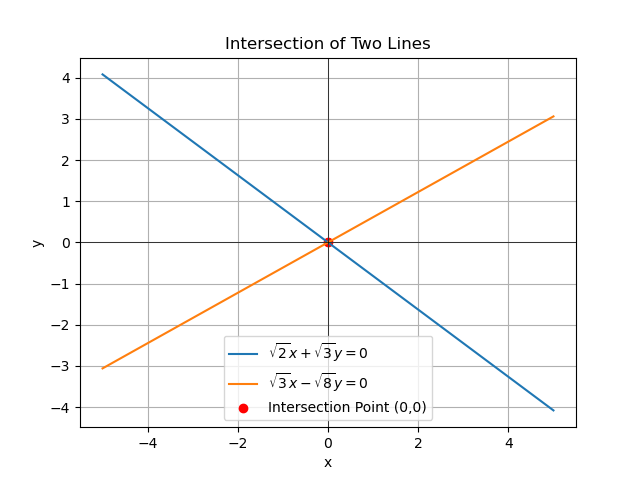
\includegraphics[width=0.8\columnwidth]{figs/10.png}
     \label{fig:1}
 \end{figure}

\end{document}